\section{Motion Planning}%
\label{sec:motion_planning}

Controllers discussed in \cref{sec:sys_iden_and_control_methods} can track a path from start to target. Providing a path is a the motion planners responsibility, motion planners seek inside the configuration space for a path from start to target configuration. A practical example of such an path is a list of successive robot poses, from starting pose (coinciding with the starting configuration) toward the target pose, where the successive poses lie close together (reachable for the robot in $\sim20$ time samples). Seeking a path from start to target inside a configuration space whilst avoiding obstacles for the robot to track is referred to as \textit{motion planning}. Finding a path between start and target configuration for pushing application avoiding collision is referred to as \textit{manipulation planning}. First this subsection presents motion planning, next subsection, \cref{sec:manipulation_planning} dedicates itself to manipulation planning. For both motion and manipulation planning sampling based methods are used, that can be discribed as.\bs

\textit{\quotes{The main idea is to avoid the explicit construction of the object space, and instead conduct a search that probes the configuration space with a sampling scheme. This probing is enabled by a collision detection module, which the motion planning algorithm considers as a “black box.”~\cite{lavalle_planning_2006}}}\bs

Generally the configuration space motion planners plan in consists of 2 subspaces, free and obstacle space. The configuration space in this thesis consists of 4 subspaces, namely free, obstacle, unknown and movable space. To solve motion planning problems for such a configuration space a dedicated motion planning algorithm has been developed that extends the existing algorithm extends the existing double tree \ac{RRT*} algorithm~\cite{chen_fast_2018}. The motion planner consists of.
\begin{center}
\begin{tabular}[t]{l p{10cm}}
$V$:& A set of nodes\\
$E$:& A set of edges\\
$P$:& A set of paths\\
\end{tabular}
\end{center}

The start connectivity tree consists of the nodes connected by edges containing the starting node, and vise versa for the target connectivity tree containing the target node. The algorithm grows the two \textit{connectivity trees} by randomly sampling configurations and adding them to the start or target connectivity tree. The algorithm explores configuration space by growing these connectivity trees. When the start connectivity tree meets the target connectivity tree a path from start to target is found.\bs

Newly sampled configurations are added is a structural manner that guarantee an optimal path is found with infinite sampling. Where optimality is defined as the path with the lowest cost. The cost is defined as a sum of a distance metric and a fixed penalty for paths that cross unknown or movable subspaces. Incentivising the algorithm to find a path around unknown or movable obstacles over path crossing through unknown or movable obstacles.\bs

The algorithm takes in 2 arguements, first the \textit{step size}, an maximal normalised distance between connected samples in the connectivity trees. Second, the \textit{search size} an subspace around newly sampled samples, inside this subspace a parent node is saught that results in the lowest cost, rewiring of closeby nodes happens and the other connectivity tree is searched to detects a full path form start to target.\bs

Now pseudocode of the proposed algorithm is provided in \cref{pseudocode:proposed_rrt_star}, functions used are elaborated on in \cref{table:functions_for_proposed_rrt_star}. The colored sections inside \cref{pseudocode:proposed_rrt_star} correspond the the surrounding colored box around subfigures in \cref{fig:motion_planner_adding_one_sample}. The following definitions are used by the proposed algorithm.\bs

\begin{table}[H]
\centering
\begin{tabular}[t]{l p{10cm}}
$x$:& A node containing a point in configuration space\\
$x_{init}$:& Creates a start and target node\\ 
$NotReachStop$:& True if the stopping criteria is not reached\\ 
$Sample_{random}$:& Creates a random sample in free-, movable- or unknown space\\
$Nearest(x, V)$:& Returns the nearest nodes from $x$ in $V$\\
$NearestSet(x, V)$:& Returns set of nearest nodes from $x$ in $V$\\
$Project(x, x')$:& Project $x$ toward $x'$\\
$CollisionCheck(x)$:& Returns true if $x$ is in free-, movable- or unknown space\\
$ObjectCost(x', x)$:& Returns a fixed additional cost if $x$ enters movable- or unknown space from $x'$, otherwis returns 0\\
$Distance(x, x')$:& Returns the distance between sample $x$ and $x'$\\
$CostToInit(x)$:& Find the total cost from $x$ to the initial node\\
$LocalPlannerCheck(x, x')$:& Return true if a local planner is able to connect $x$ and $x'$, otherwise return false. A system model (see \cref{subsec:sys_iden_and_control_methods}) acts a local planner\\
$InSameTree(x, x')$:& Returns true if both $x$ and $x'$ are in the same tree, otherwise return false\\
\end{tabular}
\caption{Functions used by the \cref{pseudocode:proposed_rrt_star}}
\label{table:functions_for_proposed_rrt_star}
\end{table}

\newpage
\begin{algorithm}[H]
\caption{Pseudocode for modified $\text{RRT}^*$ algorithm taking movable objects and constraints into account}
\label{pseudocode:proposed_rrt_star}
\begin{algorithmic}[1]

\hspace{-0.9cm}\colorbox{my_grey}{\parbox{\linewidth}{%
\State $V \leftarrow x_{init}$
\While{$NotReachStop$} 

\hspace{-0.1cm}\colorbox{my_light_blue}{\parbox{\linewidth}{%
    \State $Cost_{min} \leftarrow +\infty$ \algorithmiccomment{Create, check and project a new random sample}
    \State $x_{rand} \leftarrow Sample_{random}$
    \State $x_{nearest} \leftarrow Nearest(x_{rand}, V)$
    \State $x_{temp} \leftarrow Project(x_{rand}, x_{nearest})$

    \If{$CollisionCheck(x_{temp})$}
        \State $x_{new} = x_{temp}$
        \Else
        \State $Continue$
    \EndIf
}}

\hspace{-0.1cm}\colorbox{my_yellow}{\parbox{\linewidth}{%
    \State $X_{near} \leftarrow NearestSet(x_{new}, V)$ \algorithmiccomment{Find and connect new node to parent node}
    \For{$x_{near} \in X_{near}$}
    \State $Cost_{temp} \leftarrow CostFromInit(x_{near}) + Distance(x_{near}, x_{new}) + ObjectCost(x_{near}, x_{new})$
    \If{$Cost_{temp}  < Cost_{min}$}
            \If{$LocalPlannerCheck(x_{new}, x_{near})$}
            \State $Cost_{min} \leftarrow x_{temp}$
            \State $x_{minCost} \leftarrow x_{near}$
            \EndIf
        \EndIf
    \EndFor
    \If{$Cost_{min} == \infty$}
        \State $Continue$
    \Else
        \State $V.add(x_{new})$
        \State $E.add(x_{minCost}, x_{new})$
    \EndIf
}}

\hspace{-0.1cm}\colorbox{my_green}{\parbox{\linewidth}{%
    \State $Cost_{path} \leftarrow +\infty$ \algorithmiccomment{Check if newly added node can lower cost for nearby nodes}
    \For{$x_{near} \in X_{near}$} 
      \If{$InSameTree(x_{near}, x_{new})$} 
        \State $Cost_{temp} \leftarrow CostFromInit(x_{new}) + distance(x_{new}, x_{near}) + ObjectCost(x_{new}, x_{near})$
        \If{$Cost_{temp} < CostFromInit(x_{near})$}
           \If{$LocalPlannerCheck(x_{new}, x_{near})$}
              \State $E.rewire(x_{near}, x_{new})$
           \EndIf
        \EndIf
      \Else \algorithmiccomment{Add lowest cost path to list of paths}
          \State $Cost_{temp} \leftarrow CostFromInit(x_{new}) + distance(x_{new}, x_{near}) $ \newline\hspace*{10em} $+ CostFromInit(x_{near}) + ObjectCost(x_{new}, x_{near})$
          \If{$Cost_{temp}  < Cost_{path}$}
              \If{$LocalPlannerCheck(x_{new}, x_{near})$}
                  \State $Cost_{pathMin} \leftarrow x_{temp}$
                  \State $x_{pathMin} \leftarrow x_{near}$
              \EndIf
          \EndIf
      \EndIf
      \If{$Cost_{pathMin} == \infty$}
          \State $Continue$
      \Else
          \State $P.addPath(x_{new}, x_{pathMin}, Cost_{pathMin})$
      \EndIf
    \EndFor
}}

\EndWhile
}}
\end{algorithmic}
\end{algorithm}

\newpage
Now an example is provided of the proposed algorithm that creates and adds one sample in \cref{fig:motion_planner_adding_one_sample}. After adding the newly sampled sample is added tot the start connectivity tree, a sample is rewired then the target connectivity tree is connected to the start connectivity tree. The resulting path found can be visualised in \cref{fig:motion_planner_comparison}.\bs

\begin{figure}[H]
    \centering
    \begin{subfigure}{.49\textwidth}
    \centering
    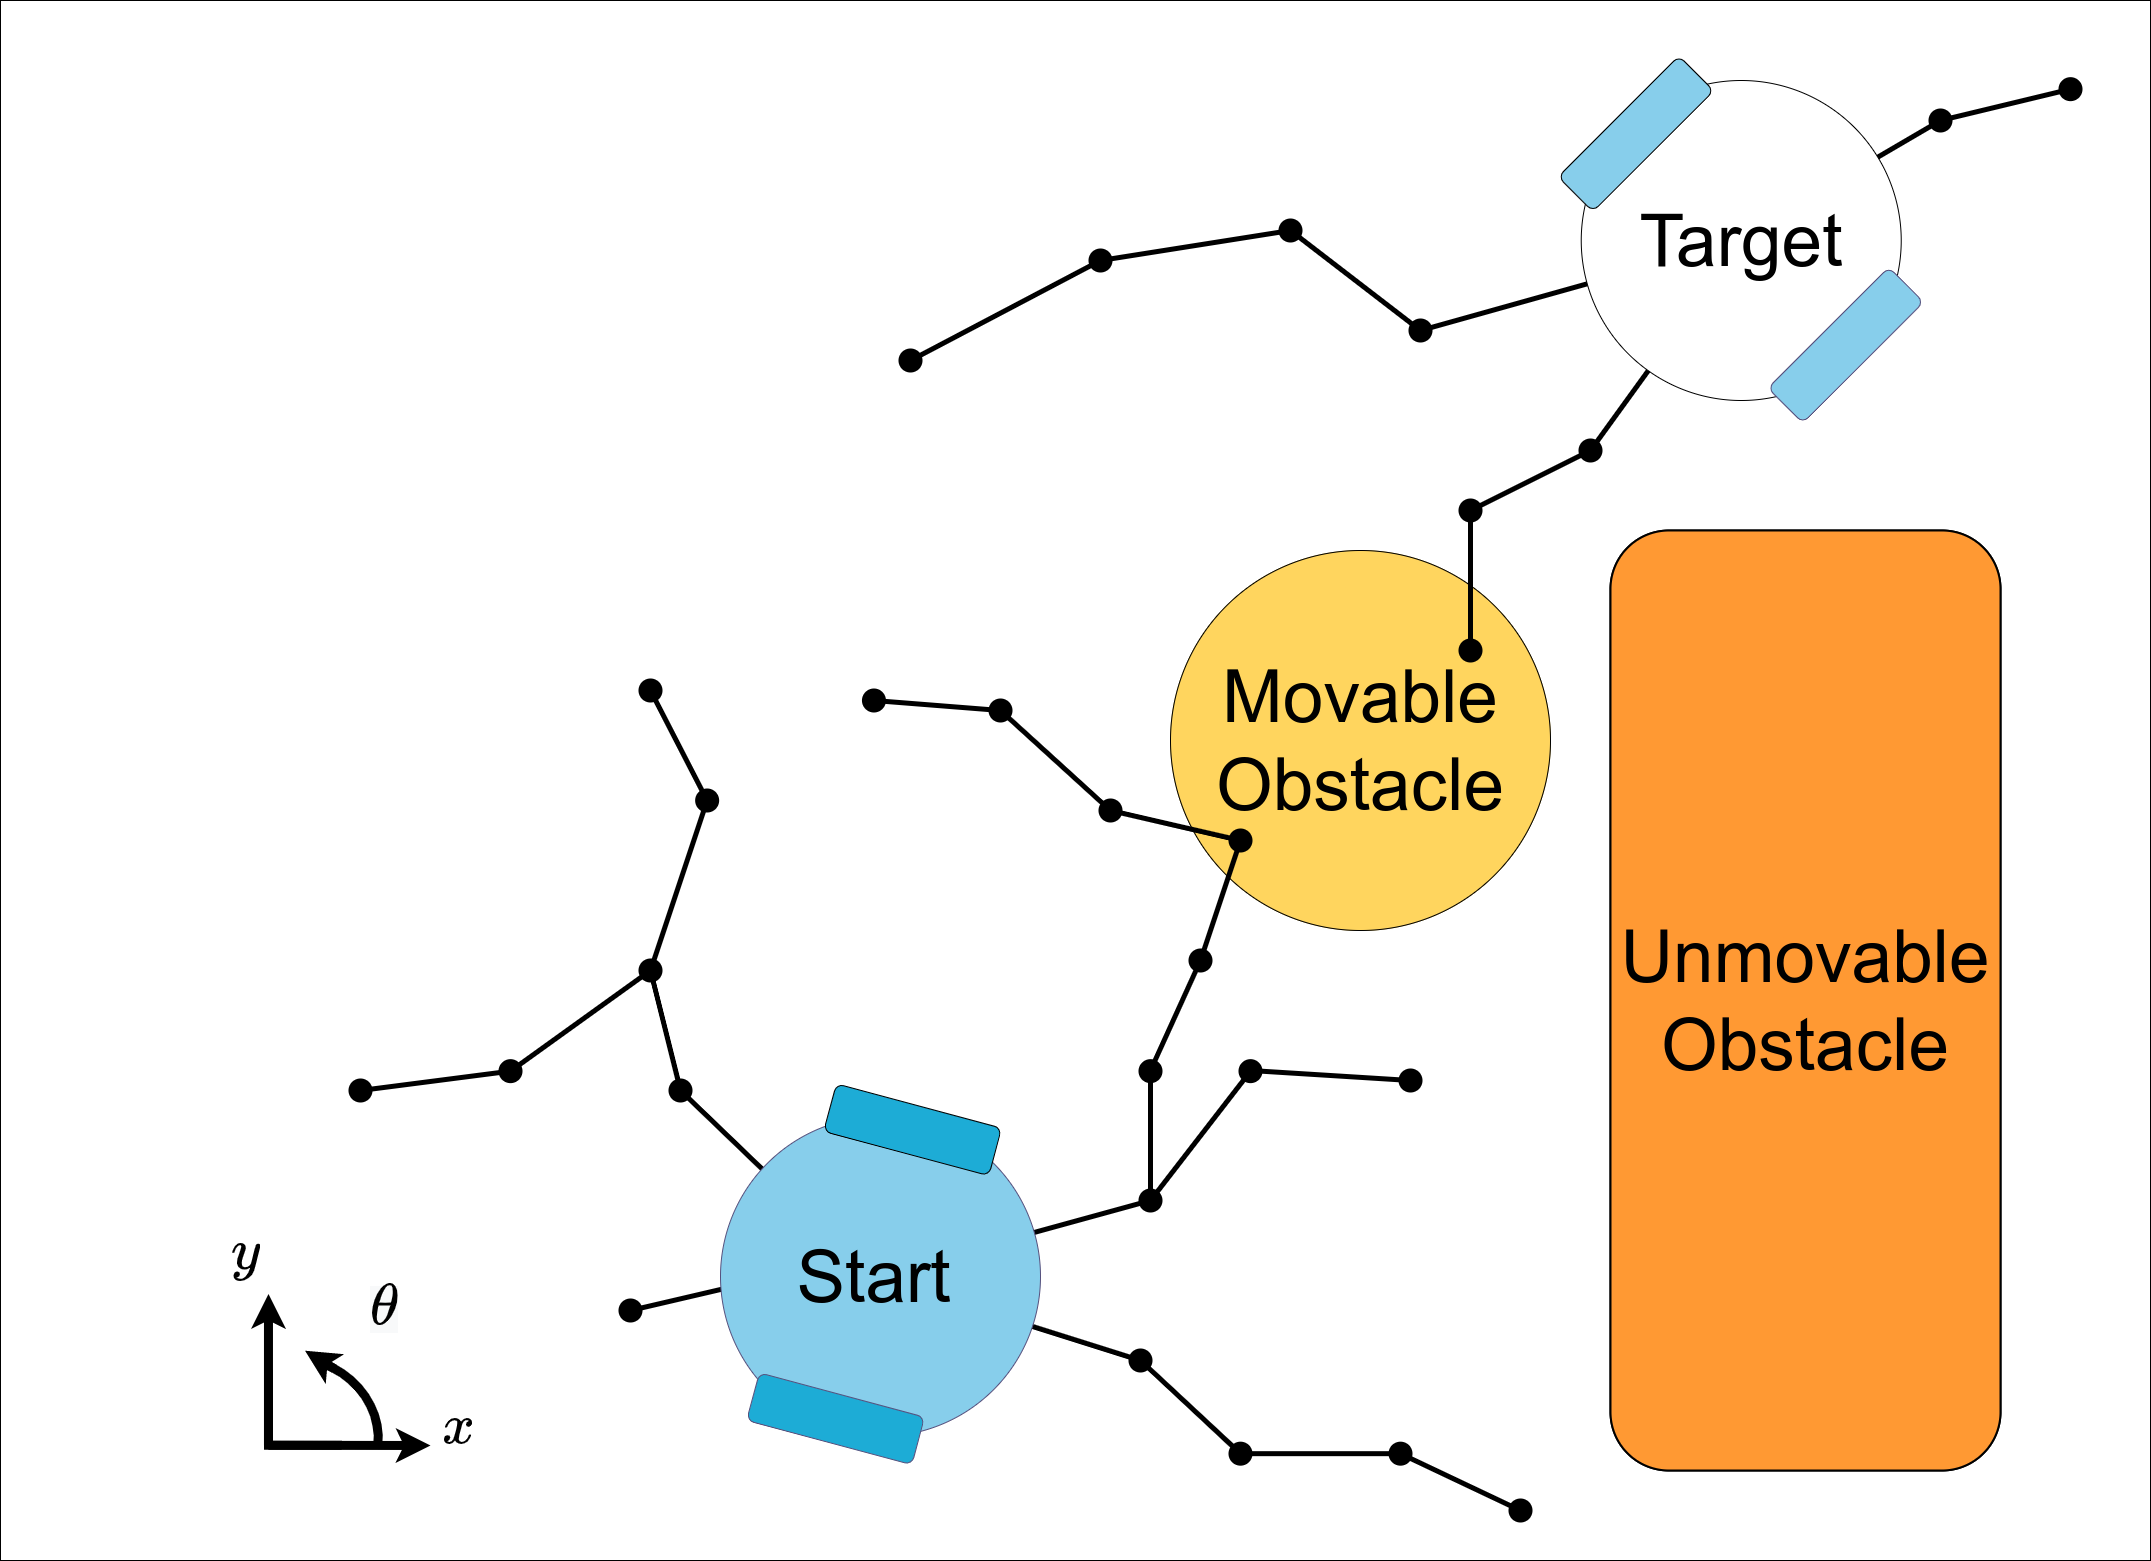
\includegraphics[width=0.93\textwidth, cfbox=my_grey 5pt 0pt]{figures/mp/1mp_init.drawio.png}
    \caption{Snapshot of the configuration space during a search\\from start to target configuration.}
    \end{subfigure}
    \begin{subfigure}{.49\textwidth}
    \centering
    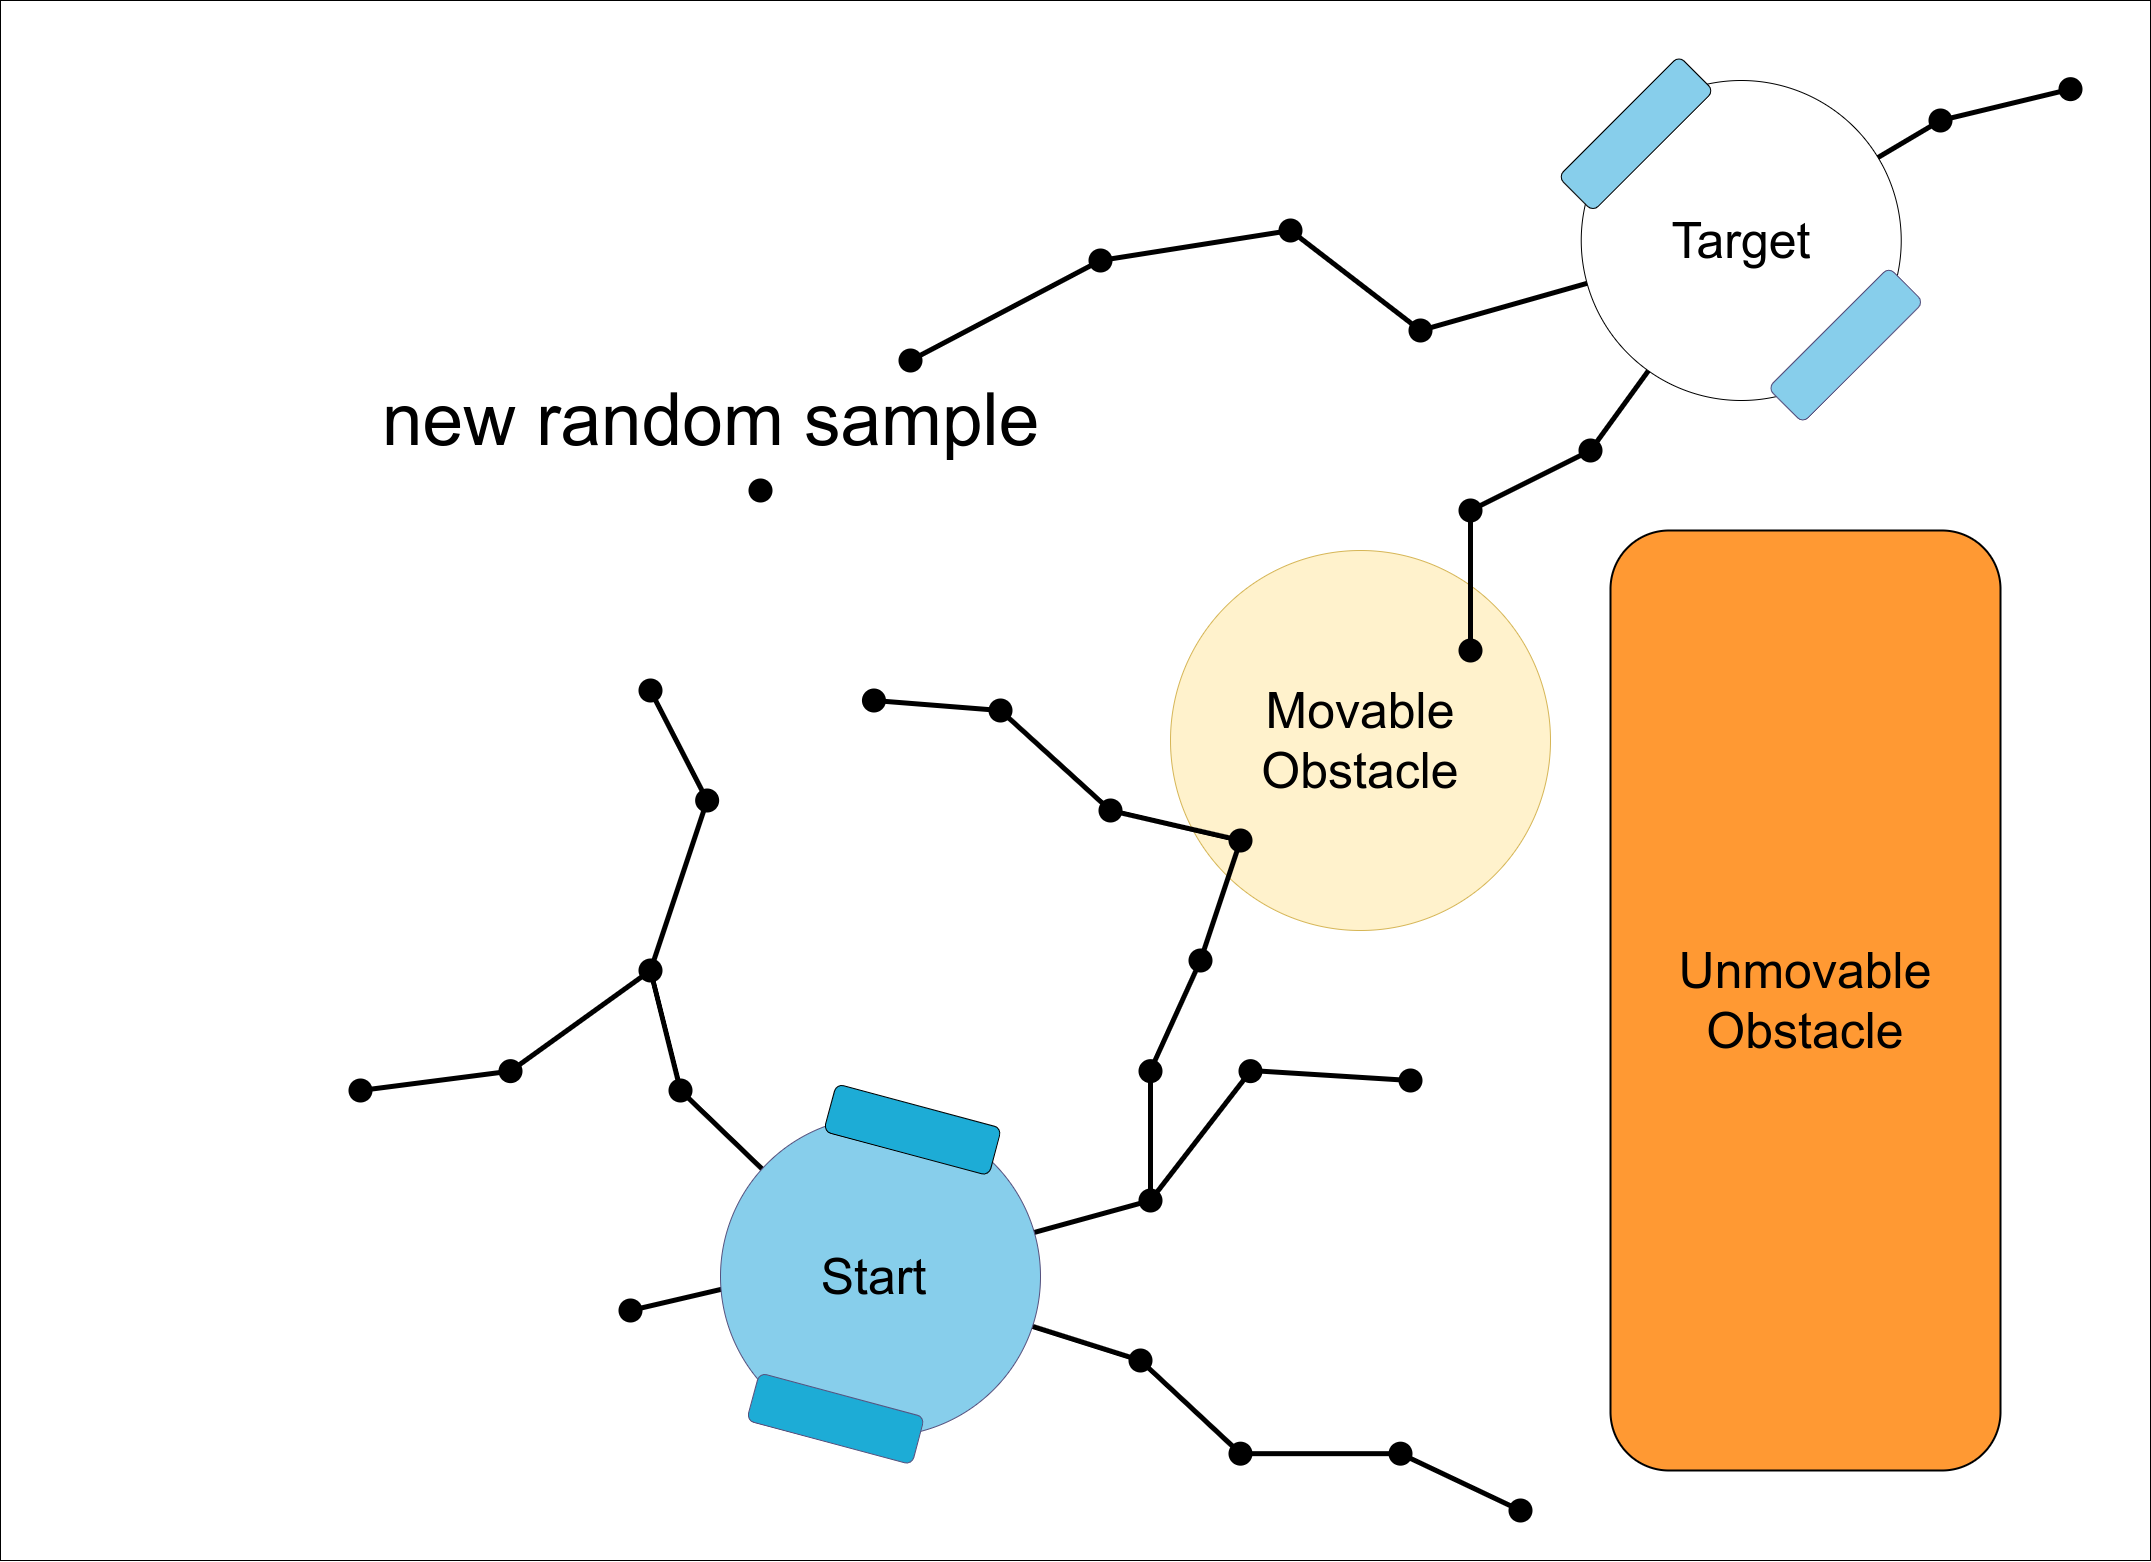
\includegraphics[width=0.93\textwidth, cfbox=my_light_blue 5pt 0pt]{figures/mp/2mp_new_rand_sample.drawio.png}
    \caption{A new random sample is generated.\bs}
    \end{subfigure}

    \begin{subfigure}{.49\textwidth}
    \centering
    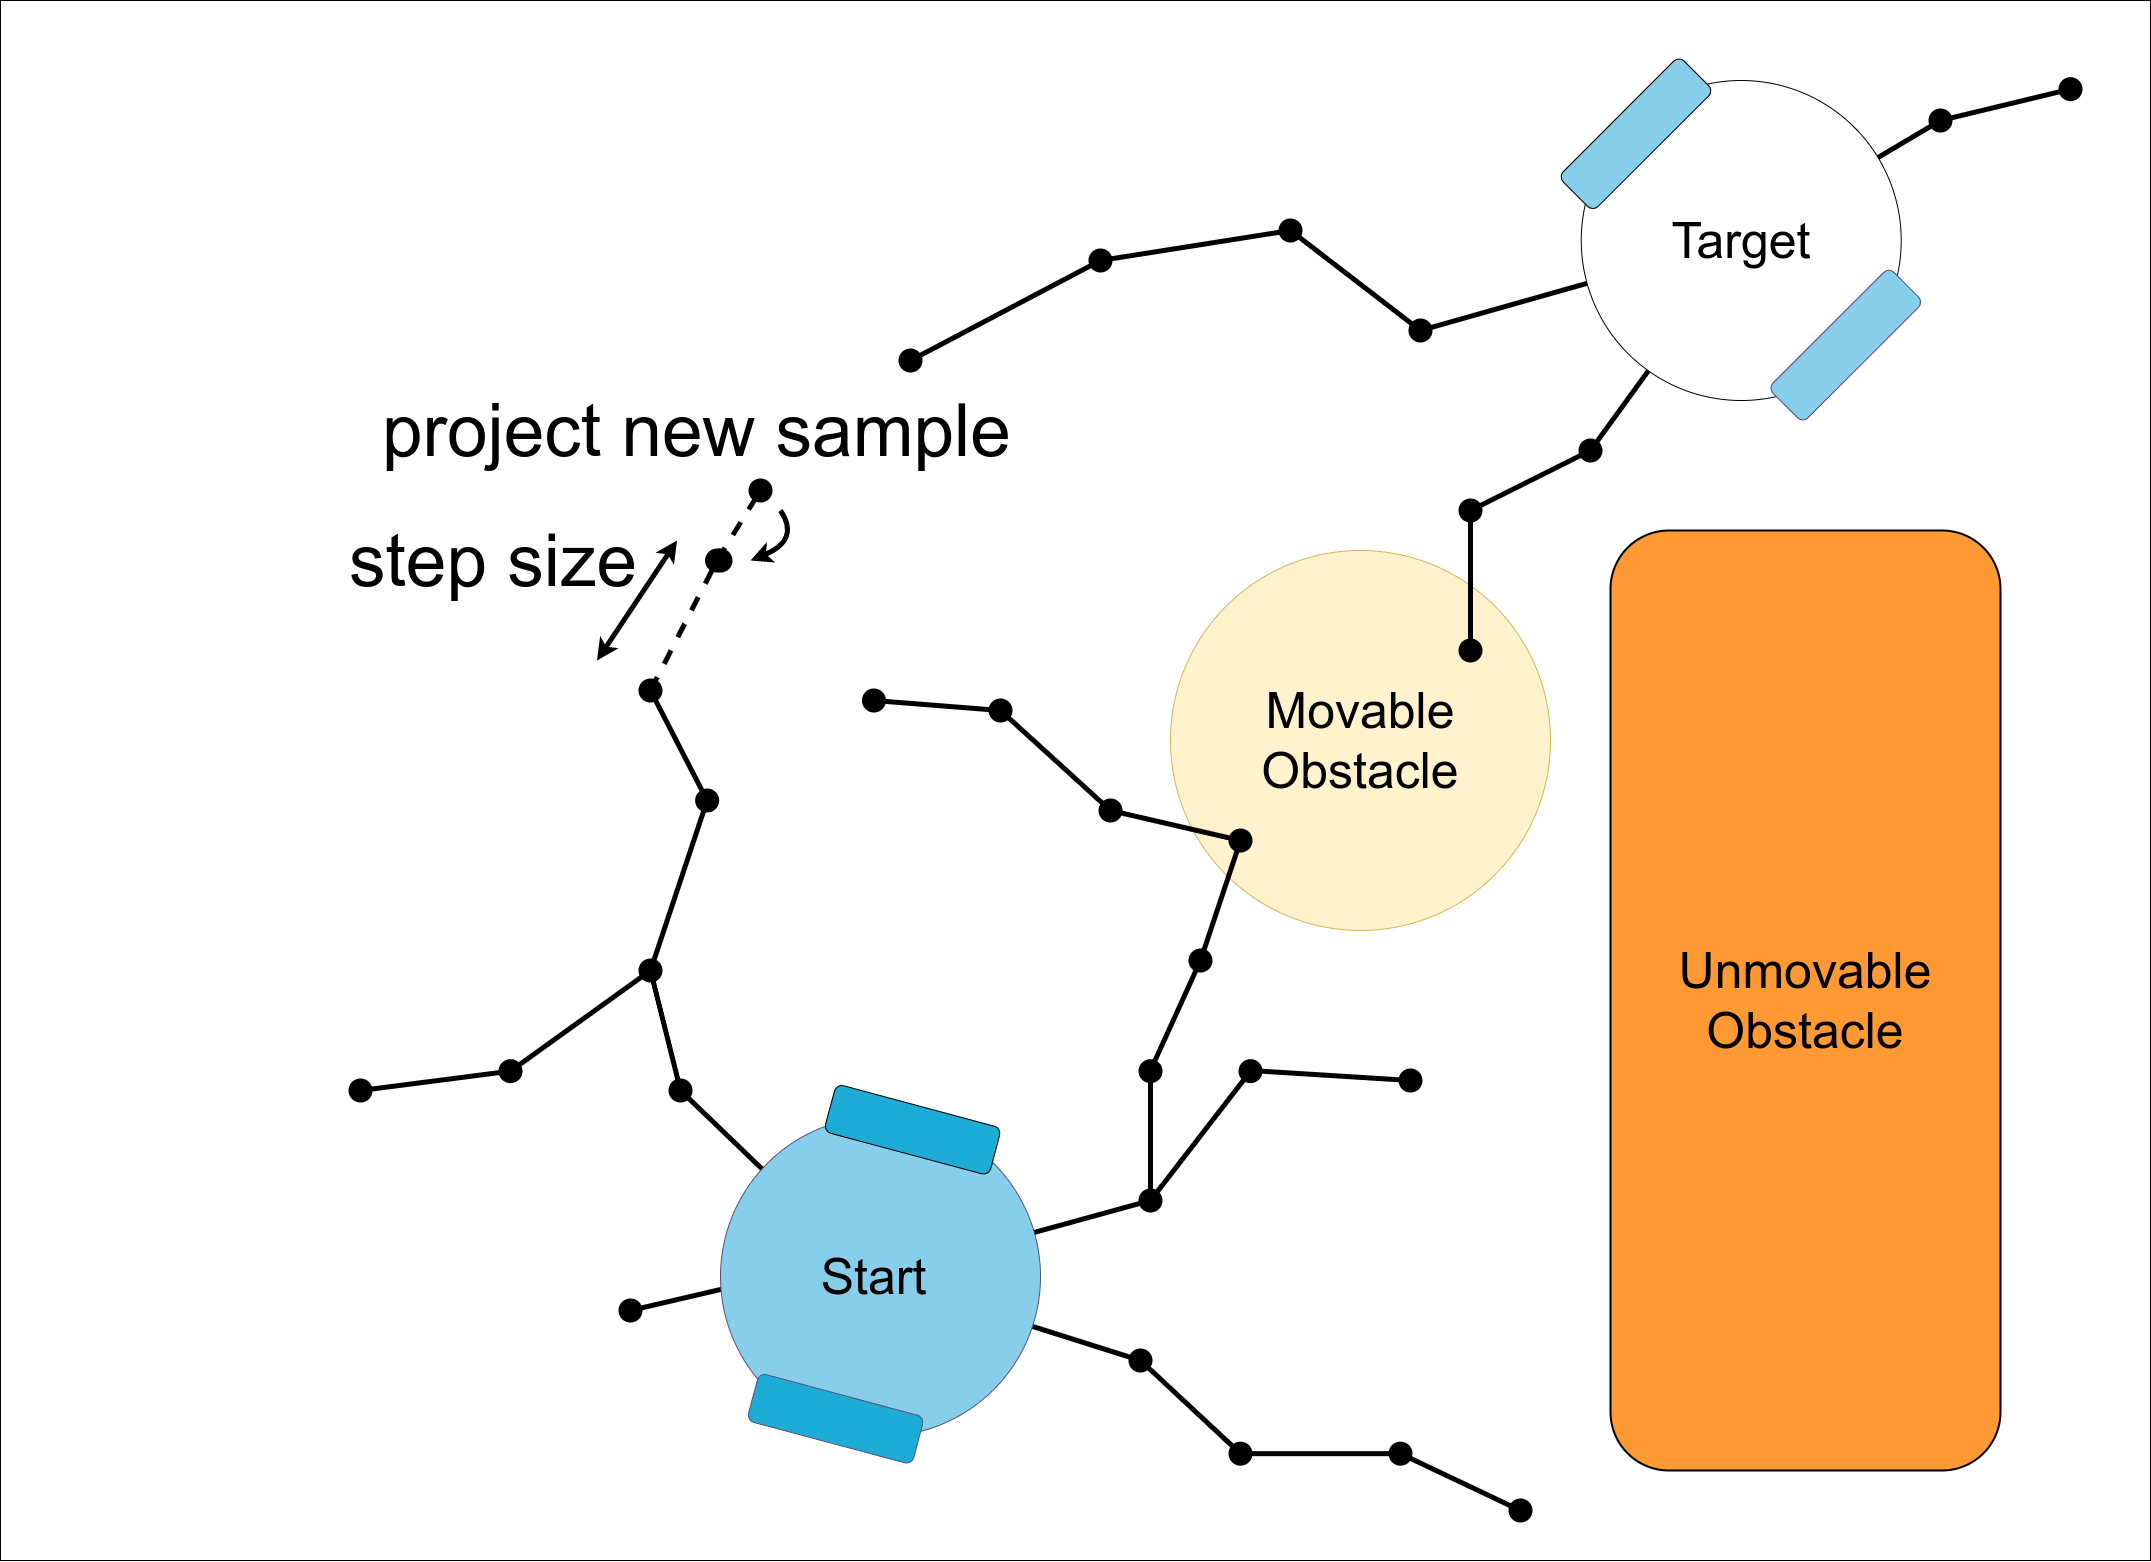
\includegraphics[width=0.93\textwidth, cfbox=my_light_blue 5pt 0pt]{figures/mp/3mp_project_sample.drawio.png}
    \caption{The new sample is projected toward the closest sample.\bs}
    \end{subfigure}
    \begin{subfigure}{.49\textwidth}
    \centering
    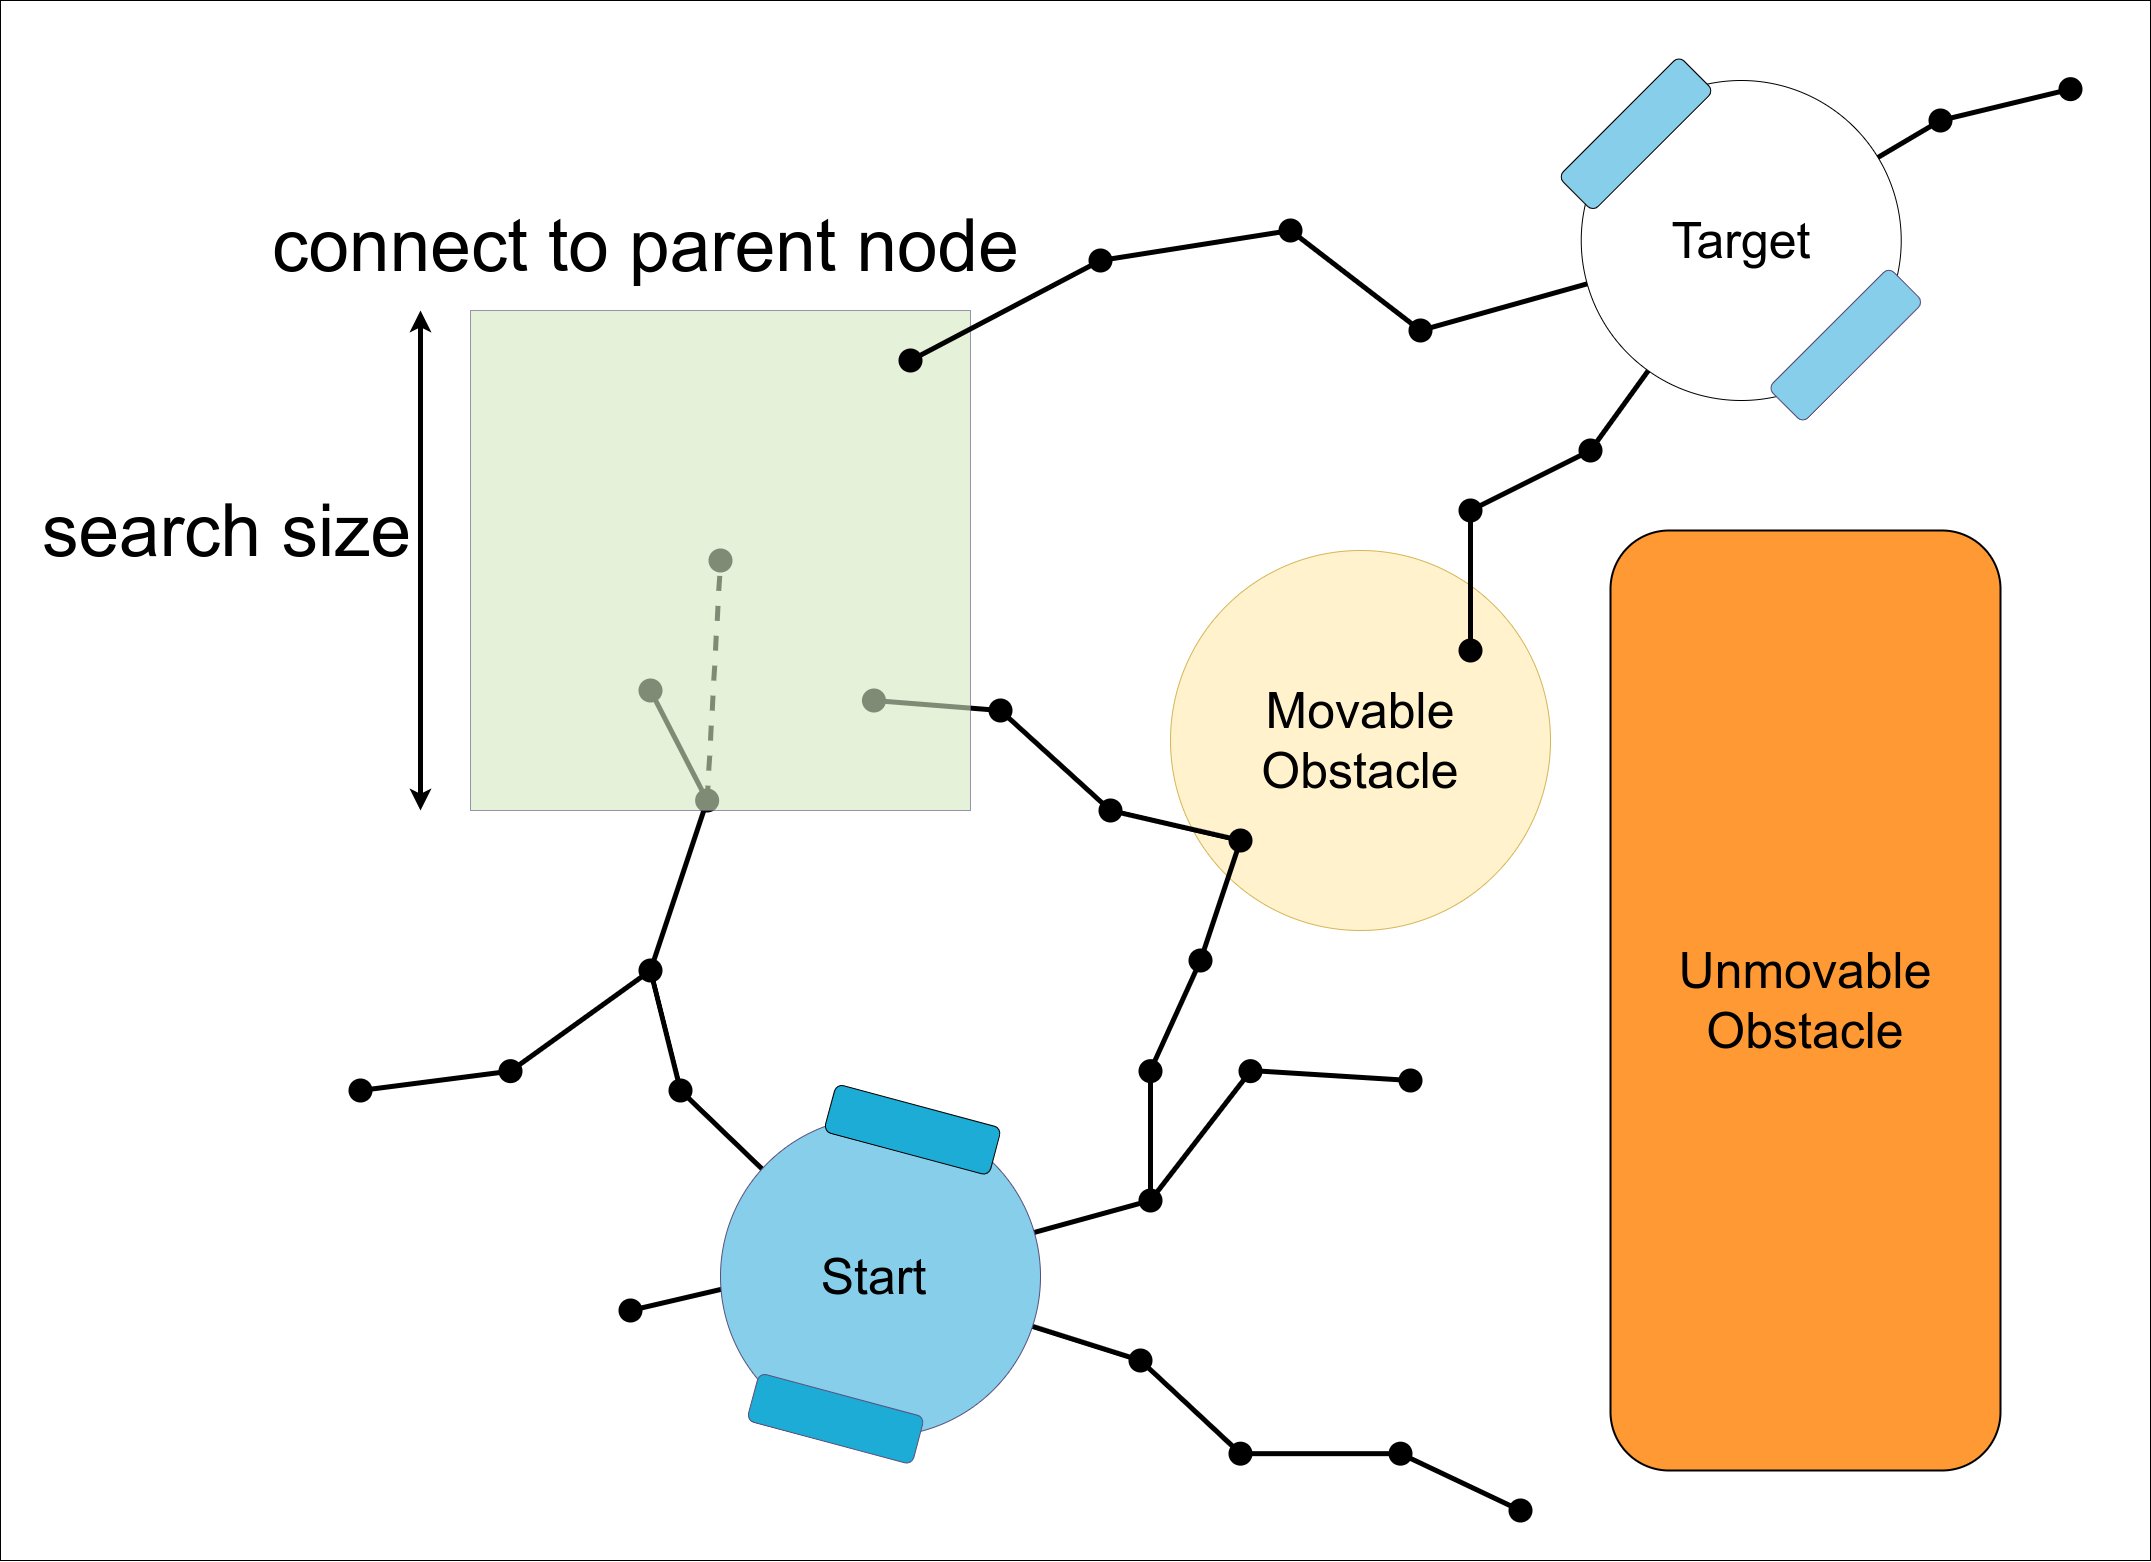
\includegraphics[width=0.93\textwidth, cfbox=my_yellow 5pt 0pt]{figures/mp/4mp_connect_to_tree.drawio.png}
    \caption{The new sample is connected to the node in search space\\that results in the lowest cost.}
    \end{subfigure}

    \begin{subfigure}{.49\textwidth}
    \centering
    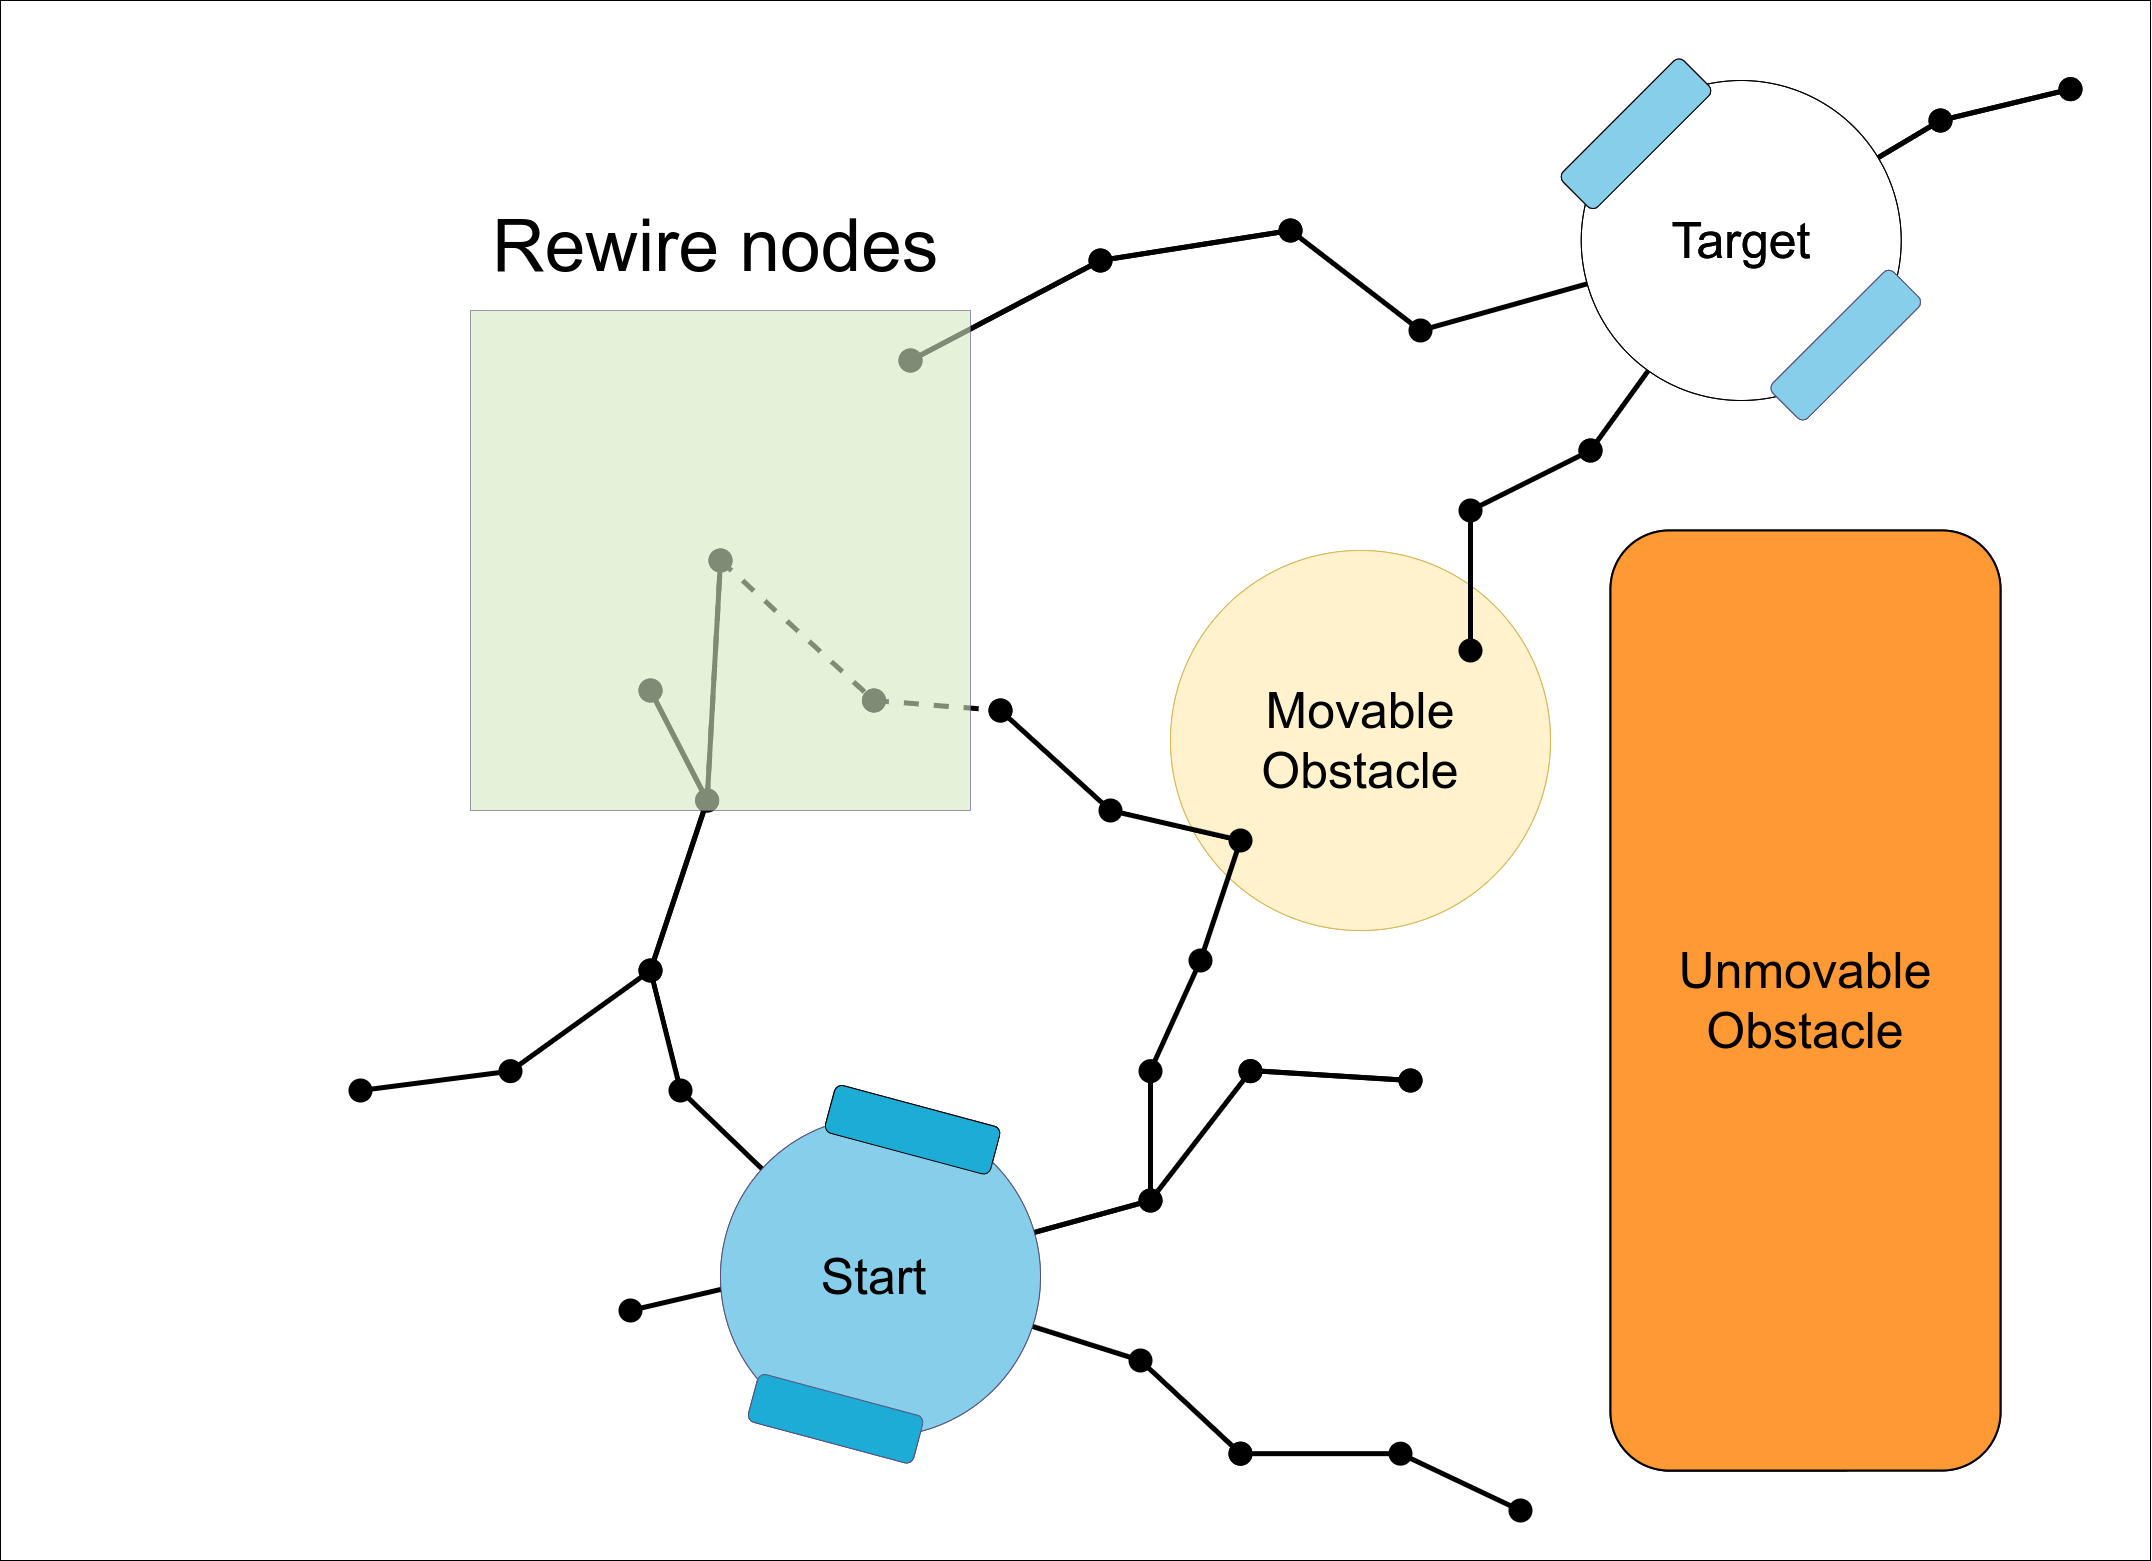
\includegraphics[width=0.93\textwidth, cfbox=my_green 5pt 0pt]{figures/mp/5mp_rewire.drawio.png}
    \caption{Nodes for which the cost can be lowered\\from the new sample are rewired.}
    \end{subfigure}
    \begin{subfigure}{.49\textwidth}
    \centering
    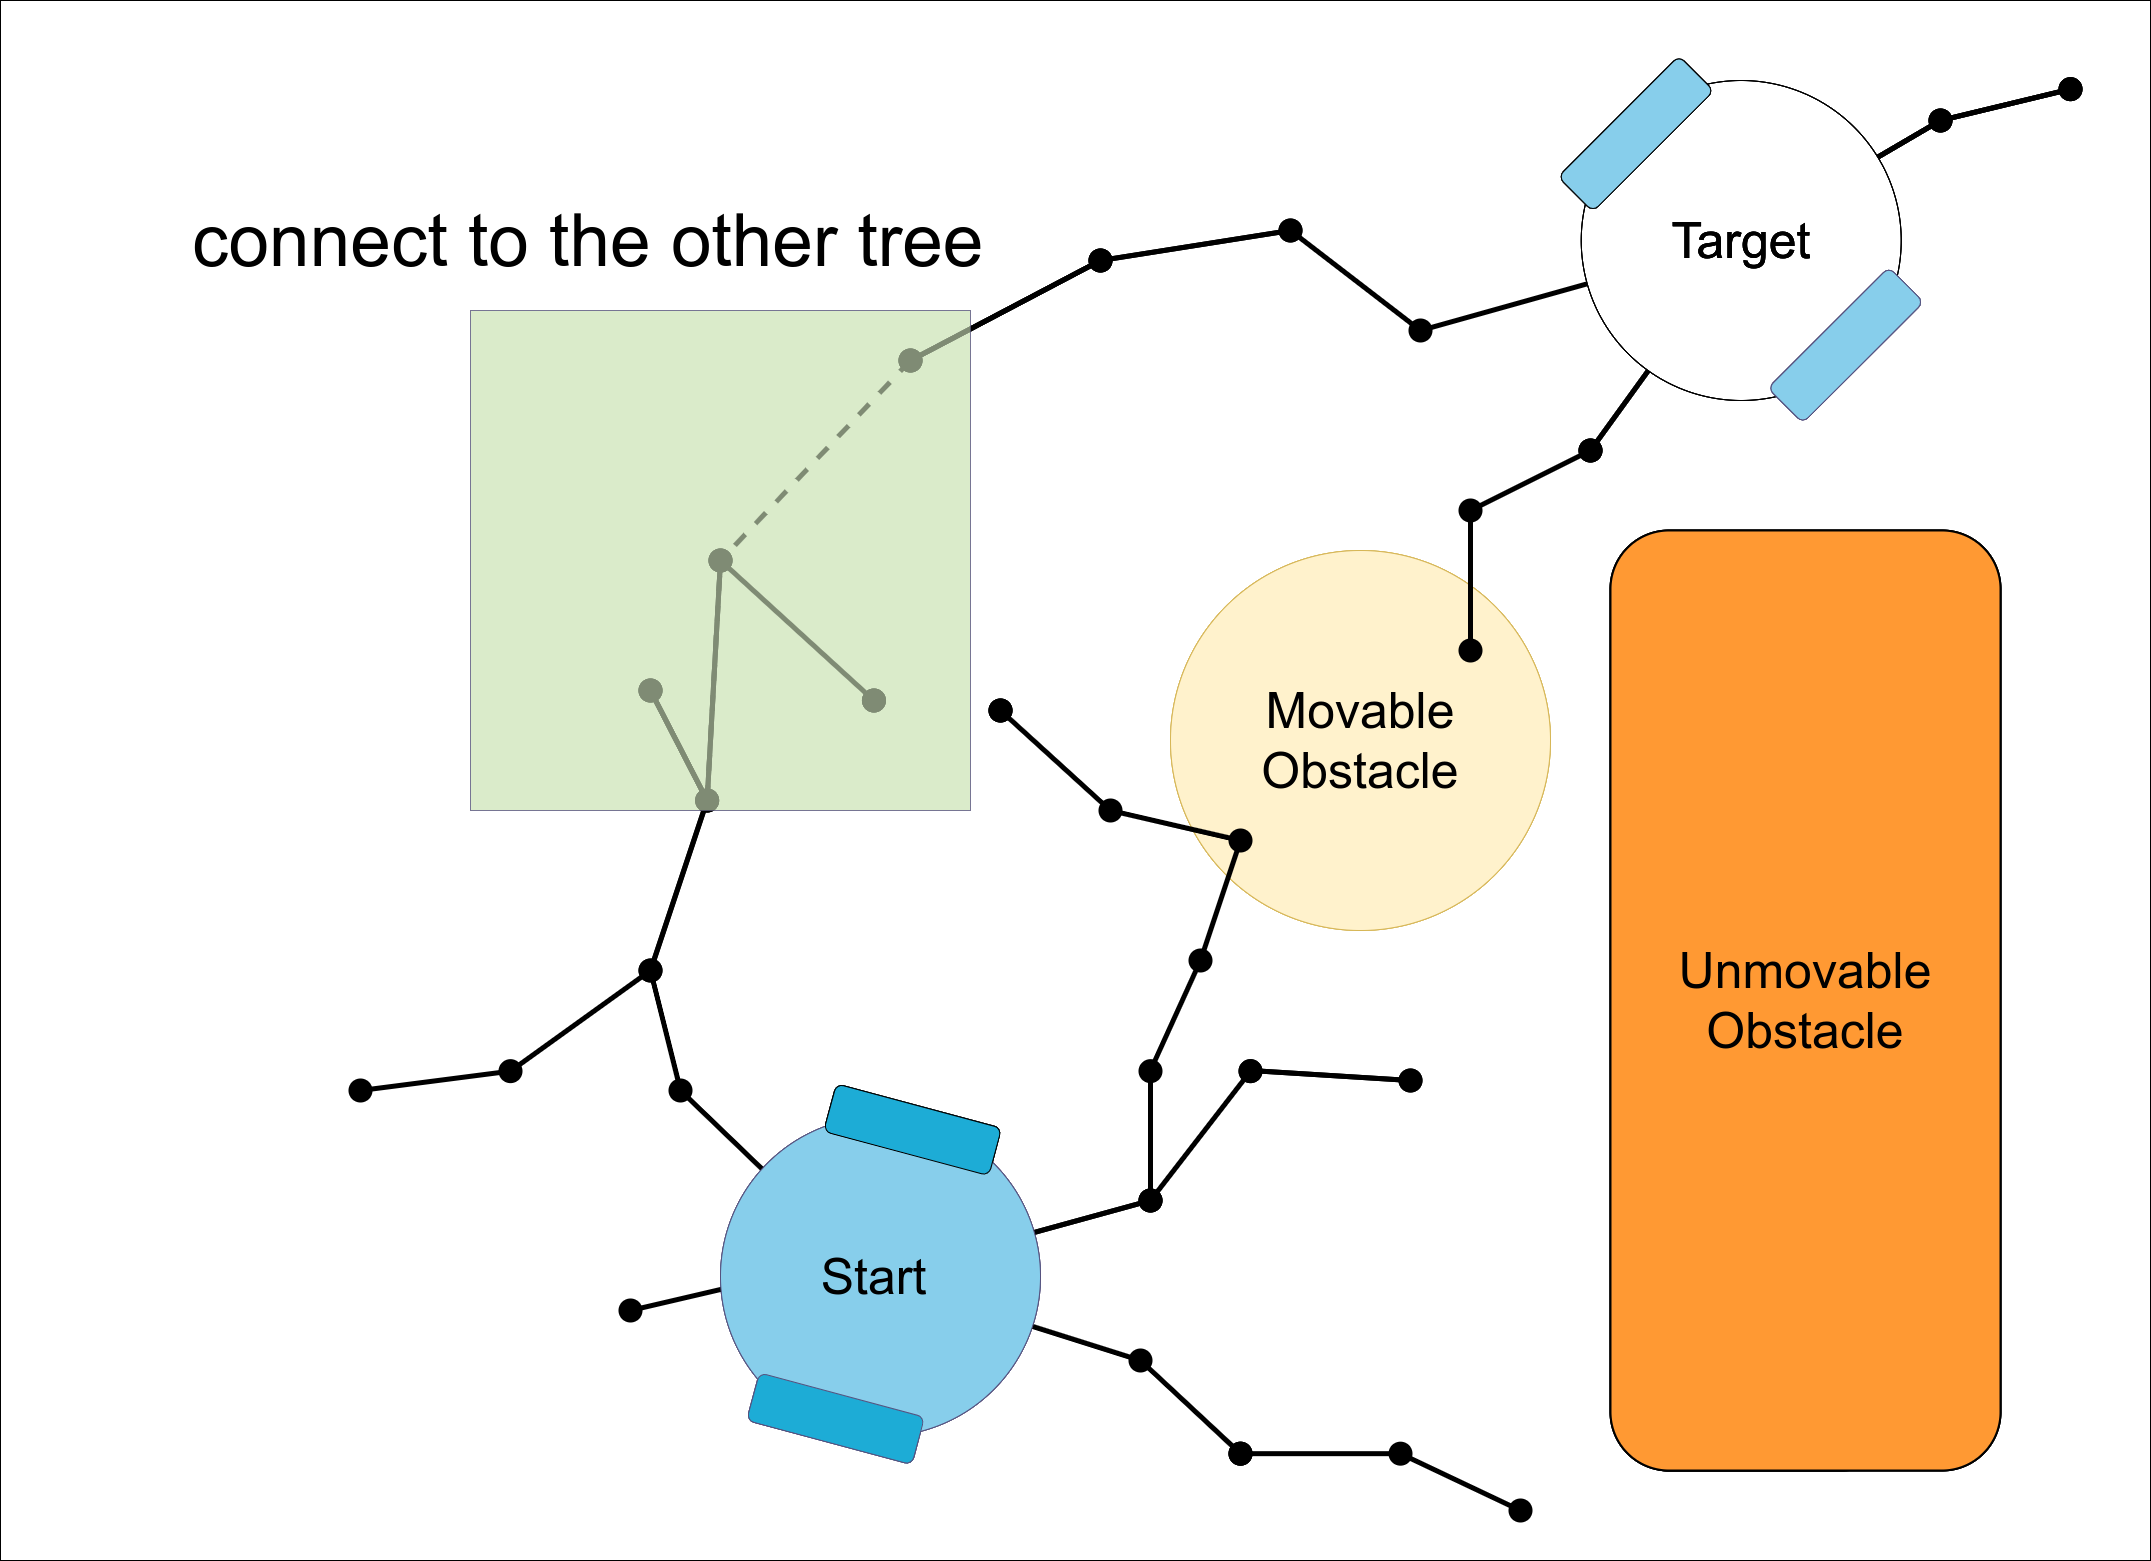
\includegraphics[width=0.93\textwidth, cfbox=my_green 5pt 0pt]{figures/mp/6mp_search_other_tree.drawio.png}
    \caption{A path from start to target configuration is found. \bs}
    \end{subfigure}

    \caption{Visualisation of the Double tree \acs{RRT*} motion planner that add a single sample to the connectivity graph. The color of the box surrounding subfigures corresponds to the colored sections in \cref{pseudocode:proposed_rrt_star}. 3 dimensional configuration space displayed as 2 dimensional configuration space ($x$ and $y$ are visable, $\theta$ is not visable).}
    \label{fig:motion_planner_adding_one_sample}
\end{figure}


\begin{figure}[H]
    \centering
    \begin{subfigure}{.5\textwidth}
    \centering
    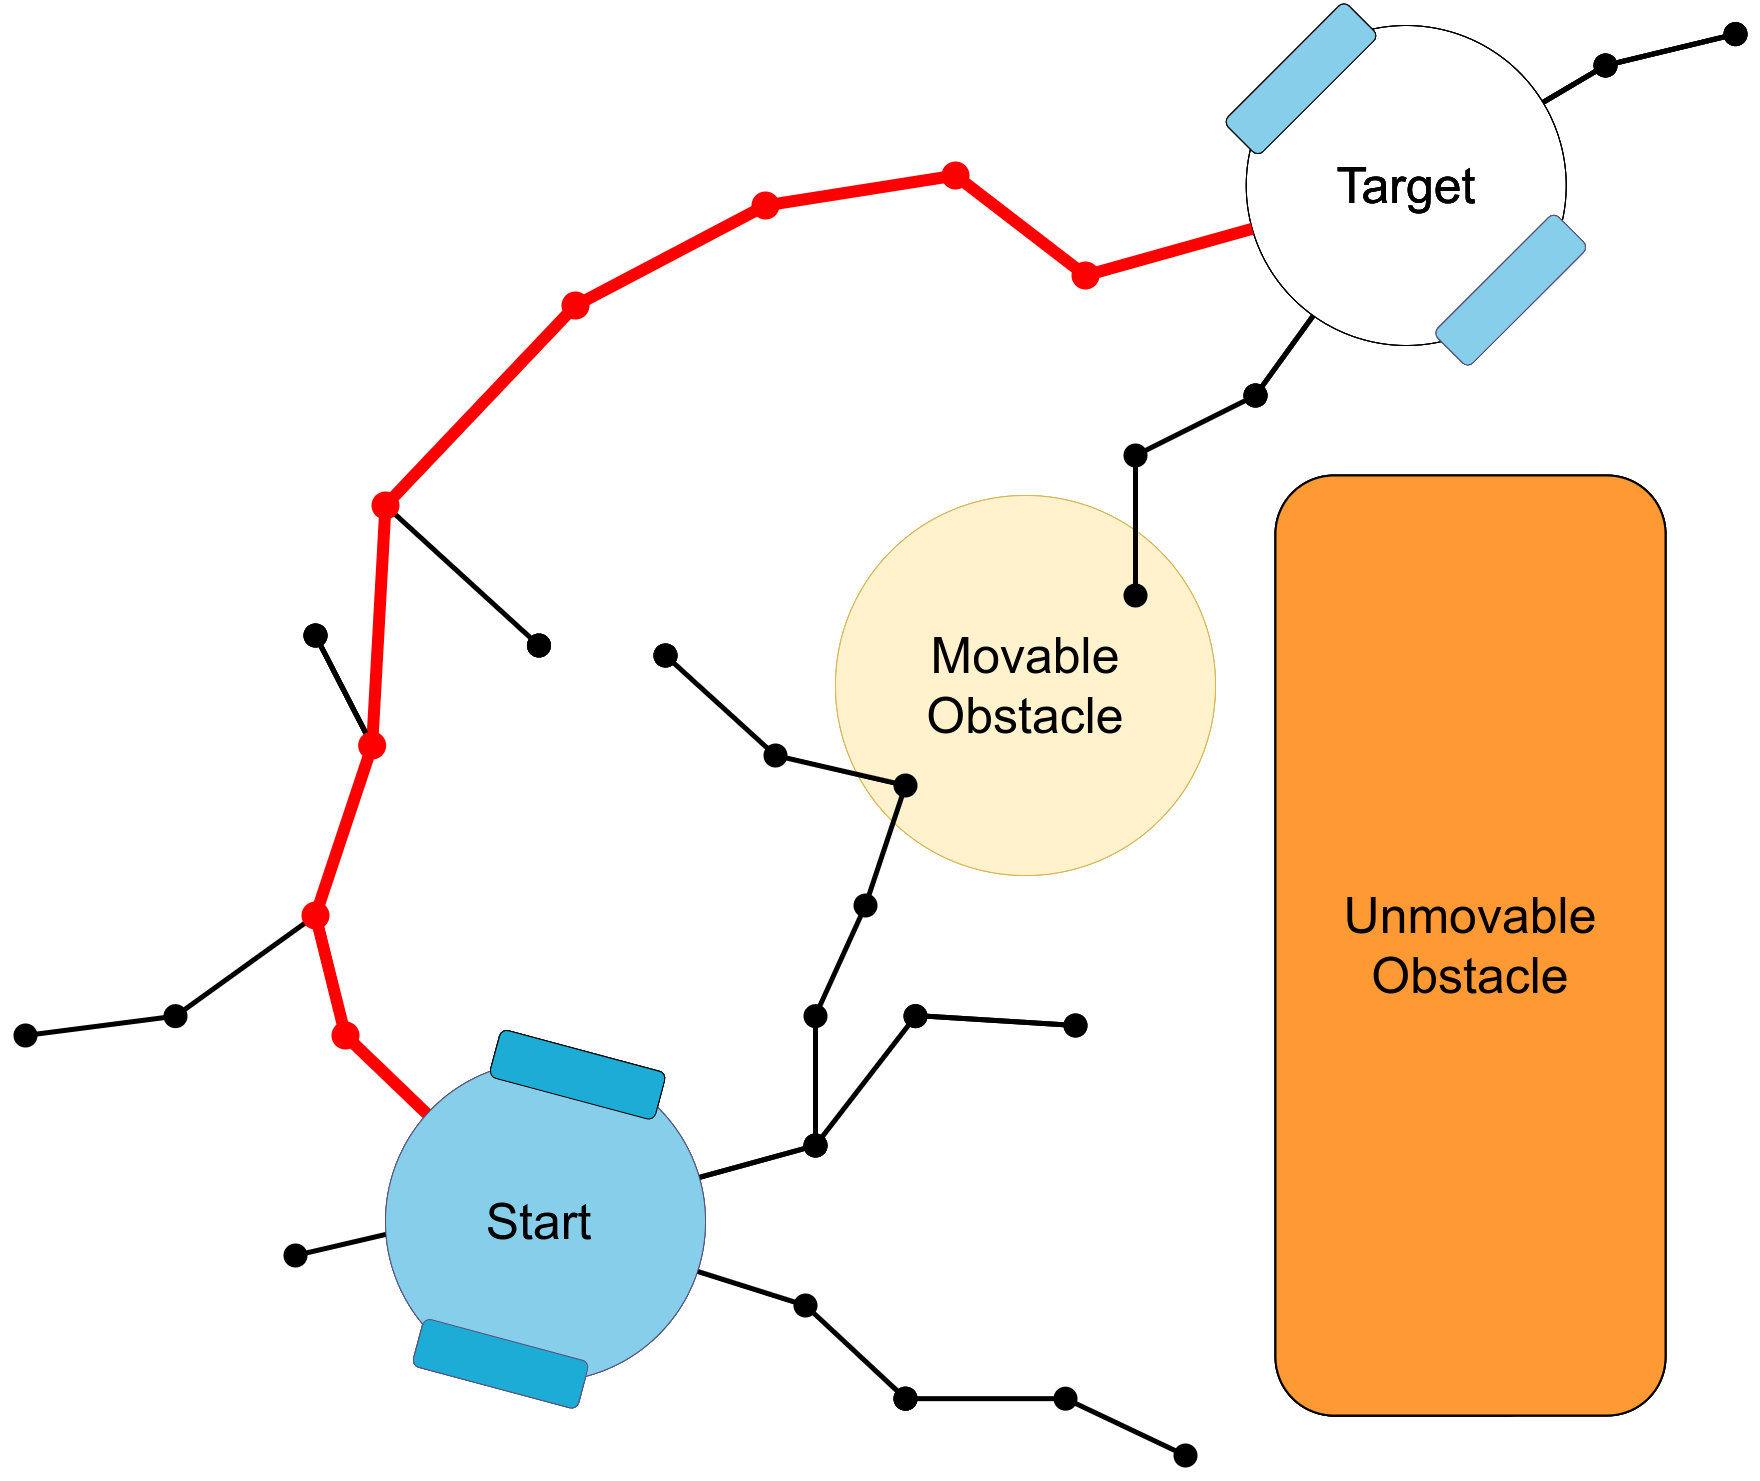
\includegraphics[width=0.8\textwidth]{figures/mp/7mp_path_found.drawio.png}
    \caption{The resulting configuration space after sample in \cref{fig:motion_planner_adding_one_sample}\\ was added. The path found is marked in red}
    \end{subfigure}%
    \begin{subfigure}{.5\textwidth}
    \hspace{-1cm}
    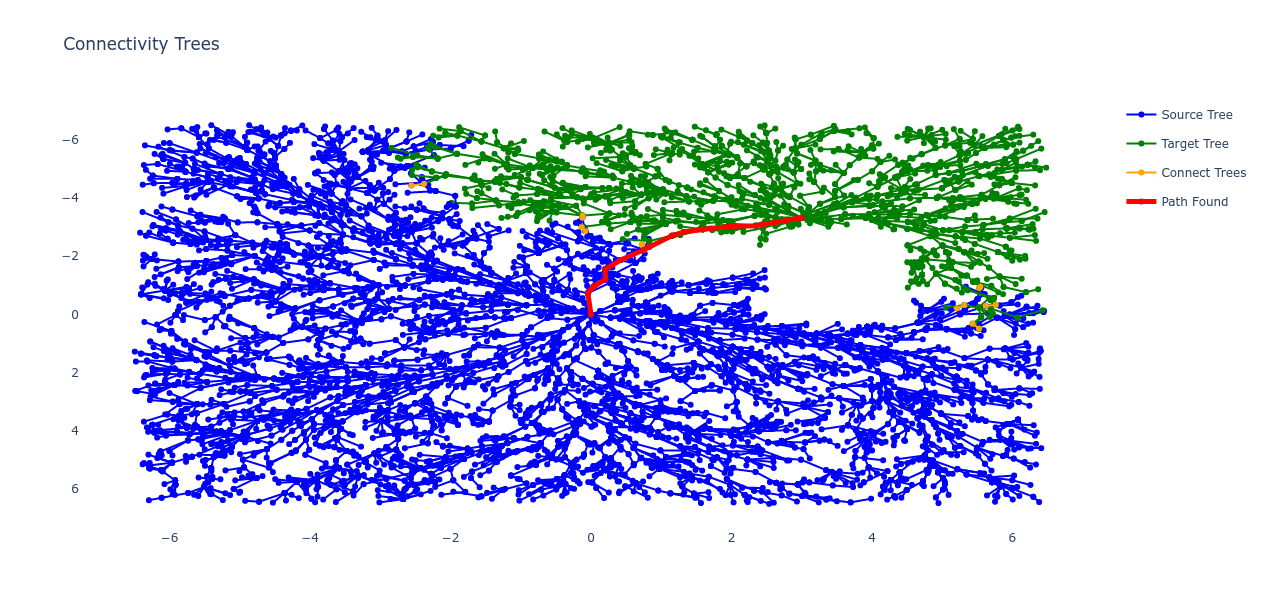
\includegraphics[width=1.1\textwidth]{figures/mp/mp_the_real_deal.png}
    \caption{A visualisation of the implemented \acs{RRT*} algorithm\\after a search from start to target}
    \end{subfigure}
    \label{fig:motion_planner_comparison}%
    \caption{Comparing schematic example to a visualisation of the real algorithm.}
\end{figure}

The result of adding an extra penalty for crossing unknown or movable subspace is that such subspaces are avoided if possible. If it is not possible to find a valid path, then movable or unknown subspaces are crossed, displayed in~\cref{fig:double_rrt_alg}. A path cannot be tracked by a controller if it crosses movable or unknown spaces, first the object must be moved, then the original path can be tracked. In~\cref{fig:double_rrt_alg} it can be seen that the motion planner cannot find a path around the movable object and is forced to add the cost to move the object. The added fixed cost for a path crossing through a movable or unknown objects motivates the motion planner to find the shortest path around objects but prefers moving an object over making a large detour.\bs

\begin{figure}[H]
    \centering
    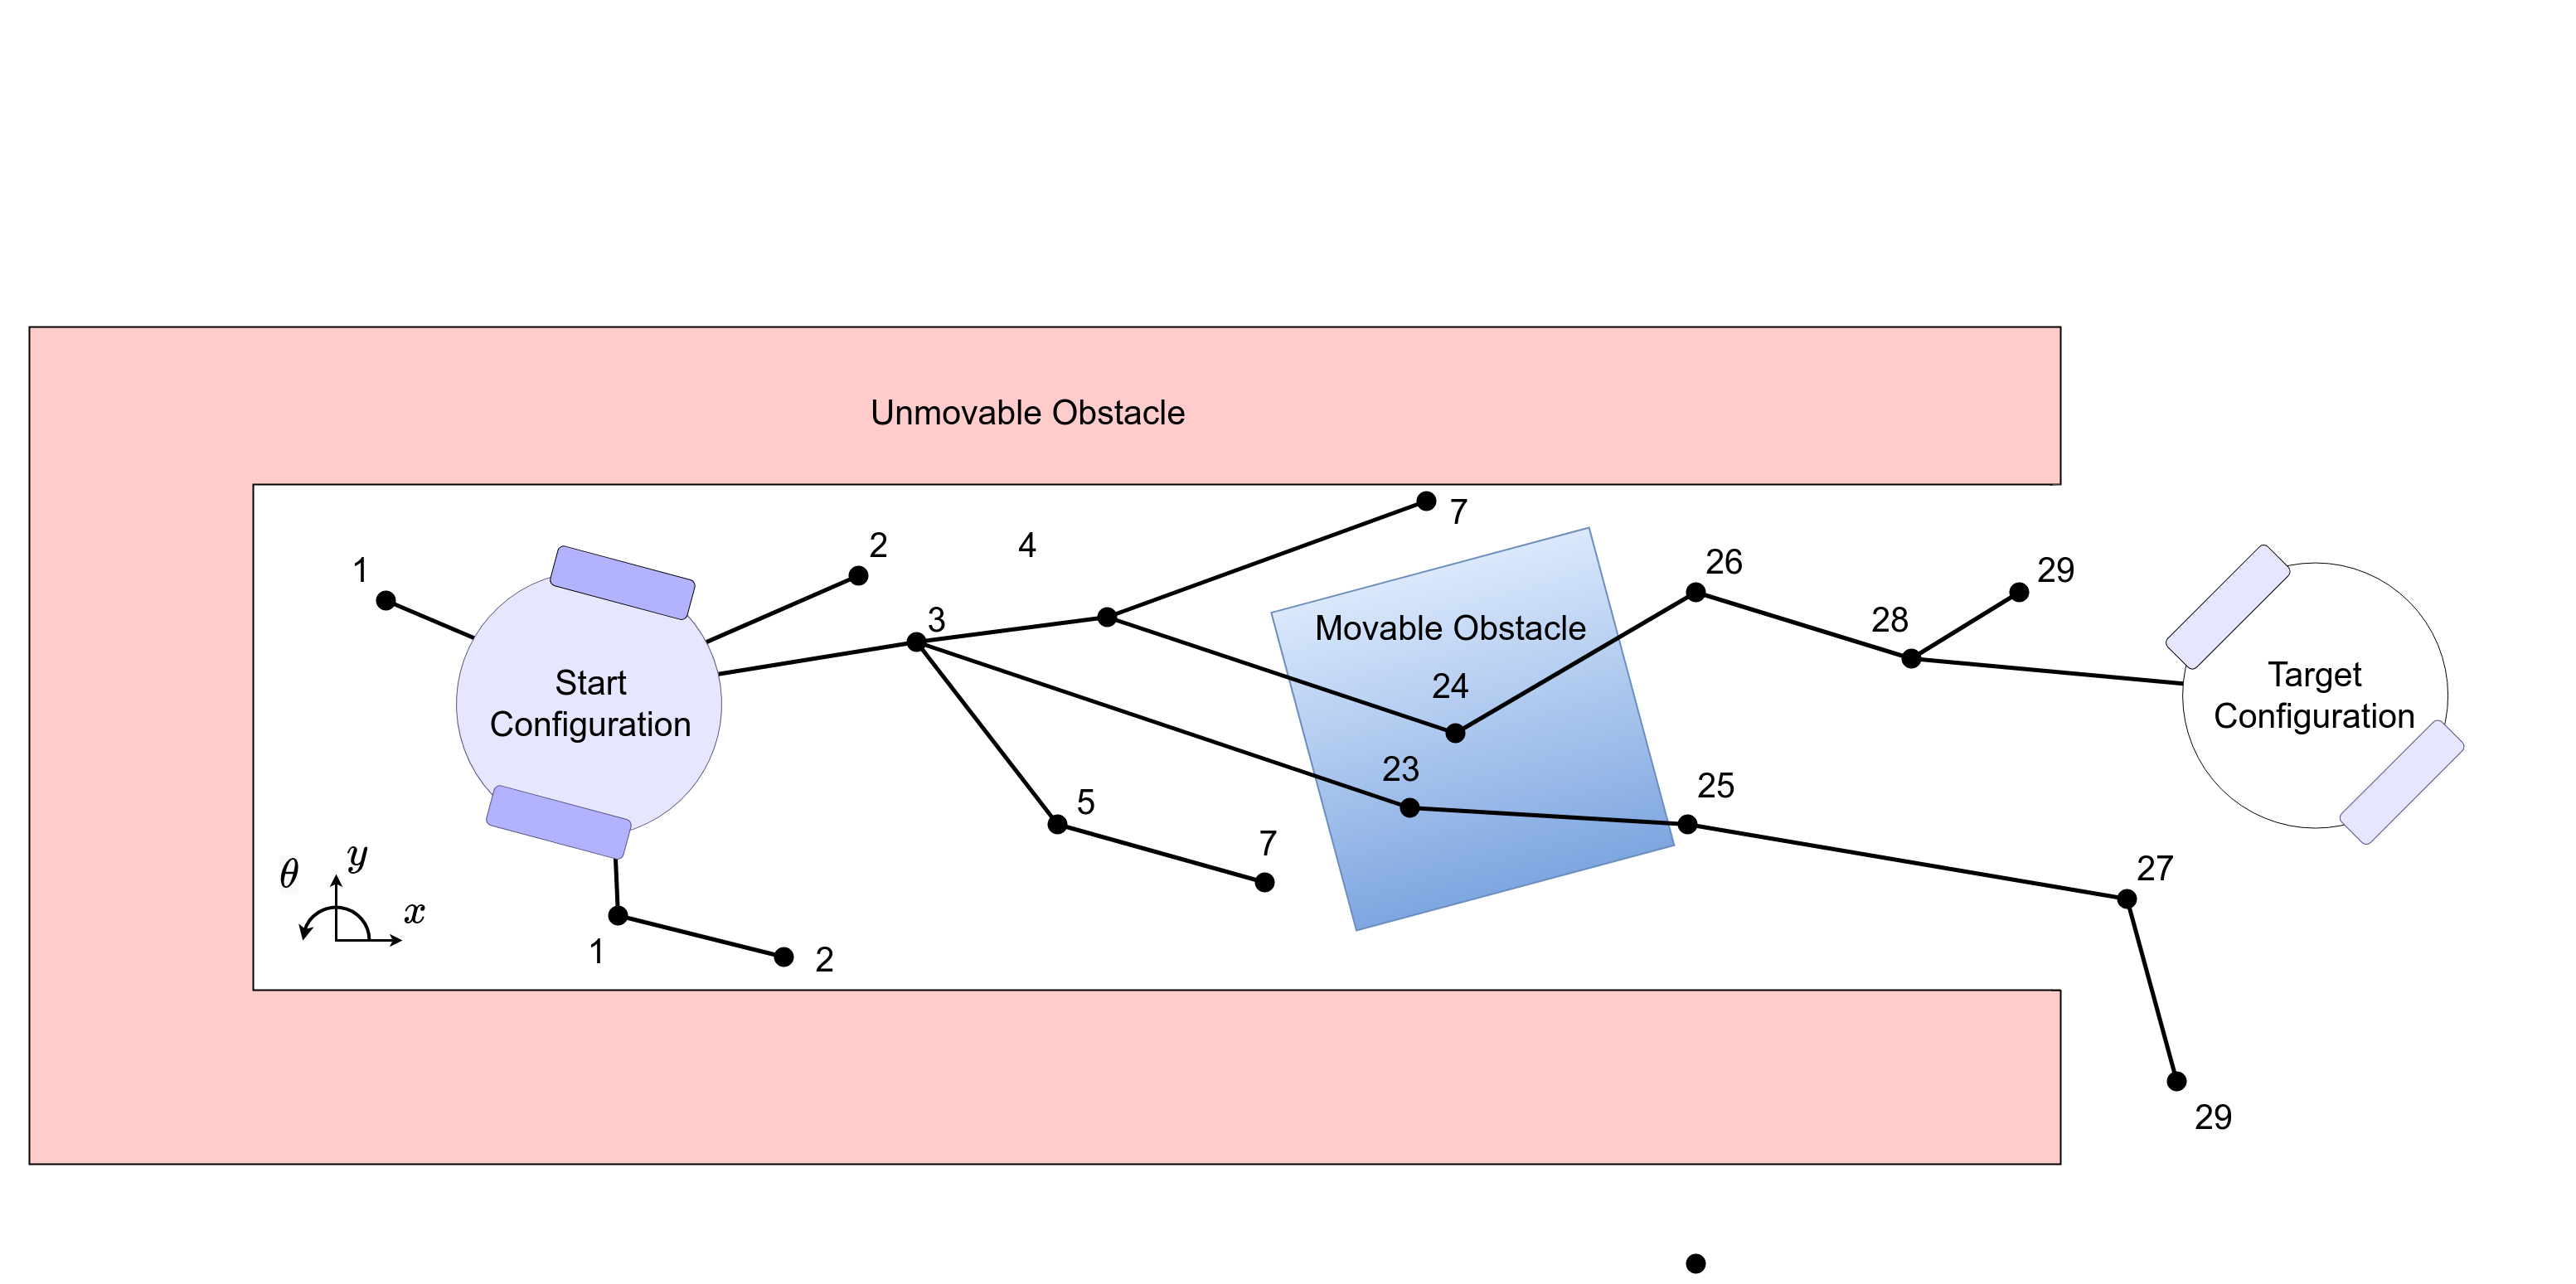
\includegraphics[width=0.9\textwidth]{figures/rrt_with_costs.png}
    \caption{Schematic view of the proposed double $\text{RRT}^*$ tree taking movable and\\unknown objects into account with cost to reach a sampled configuration displayed.}
    \label{fig:double_rrt_alg}
\end{figure}

The proposed motion planning algorithm searches the configuration space from from the start connectivity tree and the target connectivity tree. Exploring faster compared to the single tree \ac{RRT*} algorithm. The proposed algorithm rewires nodes, resulting in lowering the cost for existing paths. The proposed algorithm finds the optimal lowest cost path with infinite sampling because of it's ability to rewire nodes. The $LocalPlannerCheck$ provides paths which are feasible, such that the proposed algorithm yields paths that respect the system constraints. After all later on the system will be controlled to track the path. Now motion planning is discussed, manipulation will be discussed.
